% straditize chapter

\Chapter{Straditize}{A digitization software for pollen diagrams}

\label{chp:straditize}

\newcommand{\samplediagram}[1][false]{
	\ref{fig:sample-diagram}\hyperref[fig:sample-diagram]{
		\ifthenelse{\equal{#1}{false}}{}{#1)}}}

%----------------------------------------------------------------------------------------
%	SECTION 1
%----------------------------------------------------------------------------------------

\begin{refsection}
	
	\blockquote{
		\textit{\emph{Straditize} is published in the Journal of Open Source Software:}
		\bibforkey{SommerRechChevalierEtAl2019}
	}

\setcounter{secnumdepth}{3}
	
\begin{abstract}
	The conversion of printed diagrams or figures into numerical data has become extremely important in ensuring that scientific work, especially from the pre or early digital age, is not lost to science. One of the most common figures used in the paleo-sciences is the stratigraphic diagram, where the results of the analysis of samples are plotted against a common y-axis, usually representing age or depth. Currently this type of diagram is laborious and error prone to digitize using current software designed for simple x/y graphs. Here we present a new open source software written in python that is specifically designed to quickly and accurately digitize stratigraphic diagrams based on a user controlled semi-automatic process. The software is optimized for use with pollen diagrams, but will work well with many other types of similar diagram. The software is fully documented and includes integrated help and tutorials. 
\end{abstract}

\section{Introduction}   \label{sec:straditize-intro}

As with almost all areas of science, the digital capture, storage, manipulation and sharing of data has almost completely transformed the way that paleo-science is now undertaken compared to just 20-30 years ago. This digital transformation has created entirely new types of datasets, analysis, collaborations and visualizations, but it has also created a profound divide between the science that is available in digitized form, and that which is only available in analogue or paper form. This is a particular problem for science that was undertaken and published before this digital revolution, or where the original digital version of a dataset is unavailable, perhaps through retirement or other personnel changes, accidental damage to data storage devices, incompatible or out of date hardware storage or data file formats. 

This data however may still be available as a published or printed diagram, which can be turned into numerical data by digitization, either manually or often using graph digitizing software such as \emph{Graphclick}, \emph{Engage Digitizer}, \emph{Plot Digitizer}, \emph{g3data}, \emph{Digitizelt} and \emph{WebPlotDigitizer} \citep{Rohatgi2019}. While this approach may be optimal for simple graphs with a single x and y axis, it can rapidly become extremely time-consuming and error prone for stratigraphic diagrams with a shared y-axis and multiple x-axis. In a stratigraphic diagram the y-axis commonly takes the form of a depth or age scale (or both) reflecting sampling down a sediment core or open sediment section, which is then accompanied by a series of x-axis that plot the results of the analysis on each of these samples. Each sample may have been analyzed for a variety biotic or abiotic paleo-environmental indicators, and plotted on a variety of x-axis scales. 

Here we present an open-source software \emph{straditize} \citep{SommerRechChevalierEtAl2019} that has been specifically developed for digitizing stratigraphic diagrams. The software assumes that the figure follows the standard format associated with stratigraphic figures with a depth or age scale on the y-axis, and then a series of columns that represent the results of the analysis on common samples at specific depths or ages. The design is optimized for pollen diagrams (figure \samplediagram), but can be used without modification with any similar diagram design irrespective of the type of data being presented. The software first interprets the structure of the stratigraphic diagram and then reconstructs the data associated with each sample. This is done using a semi-automated process whereby many aspects of the software are automated but still editable by the user. The software allows the user to make continual visual checks on the digitization process, and provides the functionality to export the entire project in a data format that is independent of the platform and software\footnote{\emph{straditize} projects are exported as NetCDF file \citep{RewDavisEmmersonEtAl1989} that allows a platform and programming language independent access and sharing of the data}. The software is open-source and written in the programming language python \citep{PerezGrangerHunter2011} which makes it very flexible and easy to adapt. It is also equipped with an extensively documented graphical user interface, interactive visualizations and tutorials that allow the user to discover and to use the semi-automated methodologies. Additionally, \emph{straditize} comes with an extensive test suite for a sustainable workflow with automated checks that also ensure the basic functionality of the various features in the software.

\section{Methods: Treatment of stratigraphic diagram features}  \label{sec:straditize-methods}

\begin{figure}
	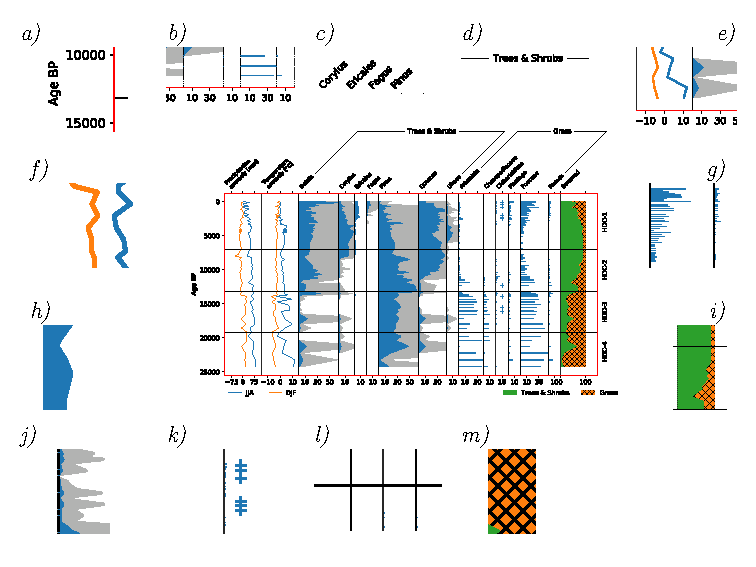
\includegraphics[width=\linewidth]{straditize-figures/sample-diagram-explained.pdf}
	\caption[Common features in a pollen diagram]{Common features in a pollen diagram. The center of the image is a pollen diagram with the data part being highlighted in red, the surrounding subfigures show some of it’s special aspects.
		Subfigures a) – e) show common features in the diagram structure, subfigures f) – i) the different plotting styles and j) – m) some of the special features. \\
		Each variable shares the same vertical axis a), is plotted as one column (sub diagram) marked by a separate vertical line b) and has a rotated title with the name of the variable c). The variables are grouped together d) and potentially have differing units on the horizontal axis  e). Common plotting styles are line diagrams f), bar diagrams g), stacked diagrams h), or  most commonly for pollen, as filled area diagram i). They may also be enhanced through exaggerations j), the visualization of taxon occurences k), horizontal lines as subdivisions of the core and vertical lines as y-axes for the columns l)  and with hatches on the area plots     for visual distinction m).
	}
	\label{fig:sample-diagram}
\end{figure}

In this section we describe the common features of a stratigraphic pollen diagram and their handling within \emph{straditize}. The emphasis is on pollen diagrams
A pollen diagram highlighting the features in a stratigraphic diagram is provided in figure
\ref{fig:sample-diagram}.

\subsection{Structure of a stratigraphic diagram}  \label{sec:straditize-structure}

\subsubsection{Stratigraphic columns}  \label{sec:straditize-strati-columns}
A stratigraphic diagram consists of multiple sub diagrams, each visualizing one or more different variables, for example the percentages of different pollen taxa, the concentration of different chemical elements, or the various percentages of different grain sizes. These sub diagrams share one common axis which is usually the age or depth of the core (see fig.~\samplediagram[a]). 
The diagram is then divided into multiple sub diagrams which we refer to as the columns of the stratigraphic diagram (fig. \samplediagram[b]). Each column visualizes the data of one variable, such as a pollen taxon, or multiple variables where these are plotted within the same column (same x-axis), such as winter and summer precipitation shown in the left most column of figure \samplediagram. The current version of \emph{straditize} requires that the columns do not overlap and that multiple variables plotted in the same column do not overlap either. The software can process multiple variables in a column so long as these are stacked or additive, and therefore they never overlap. An example in a pollen diagram could be where multiple species of, for instance Betula, are plotted as a stacked diagram in a single column so that the sum of the species also shows the total Betula.  

At the top of each column it is usual to find the name of the variable plotted in the column. This may be shown at a variety of angles, but usually either vertically, or at an angle or rotated to make it easier to read and fit within the diagram (fig. \samplediagram[c]). This label can be automatically read by \emph{straditize} and the name assigned to the respective column data, although care should be taken as the label is sometimes offset from the column it represents.  

Variables are also often grouped together and the group labelled, for instance in pollen diagrams into \emph{trees \& shrubs}, and \emph{herbs} (fig.\samplediagram[d]). For pollen data these groups usually share the same x-axis units/scaling (as in fig.\samplediagram[b]). In \emph{straditize} the units/scaling can be set and applied to a whole group of columns/variables, or set and assigned for each individual column/variable (see fig.\samplediagram[e]).

\subsubsection{Diagram types}  \label{sec:straditize-types}
A number of different diagram types are shown in figure \samplediagram\, that are commonly used in pollen diagrams, as well as other stratigraphic diagrams. These can all be identified and read by \emph{straditize}. One of the most commonly found diagrams in pollen diagrams are line diagrams (fig.\samplediagram[f]), or line diagrams where the area underneath of the line is filled to make an area diagram (fig.\samplediagram[h]). Data is also often commonly presented as bar diagrams that make it clearer where the individual samples are located (fig.\samplediagram[g]). Both bar and line/area diagrams may also be stacked, where (as we have already mentioned) columns may contain multiple variables stacked one upon the other (fig.\samplediagram[i]). These various diagram types require different digitization strategies, which we discuss in the digitization section below (see section \ref{sec:straditize-digitization}).

\subsubsection{Informative features}  \label{sec:straditize-features}
Other more specialized features can also be found in pollen diagrams that provide additional information for the reader, but are more difficult to interpret for the software. For instance the taxa or variables in a pollen diagram are usually all plotted on the same scale even if they are in different columns, so that direct visual comparison can be made between them. However, whilst this works well for large percentage values, it can often be difficult to see changes in low percentage values, which may still be ecologically important. To help the reader see these changes in low percentages, pollen diagrams often include a vertical exaggeration. This means that the percentages for a pollen taxa in a column will be plotted with two lines, one showing the percentage value shown on the scale, and the other showing the percentage value multiplied or exaggerated by a certain factor (usually 5 or 10) (fig. \samplediagram[j]). A different approach to the same problem is to mark the low percentages with a symbol or marker. For instance, a common method is to mark all samples with less than 0.5\% or 1.0\% with a \enquote{+} symbol (fig. \samplediagram[k]).

Other features that are often added to pollen diagrams and other stratigraphic diagrams are vertical and horizontal lines. Vertical lines often denote the start of a column, representing the baseline of the y-axes. These are often a continuous or discontinuous dashed line, and when it is quite a thick line it can be difficult to define its position relative to the x-axis. Horizontal lines usually run across columns and are often used to denote different sections of the diagram. For instance, in pollen diagrams they are often used to denote zones or sections of the diagram that have a similar ecological assemblage. These horizontal lines do not usually provide useful numerical data and their intersection with column lines can make reading the column lines more difficult for the software. Another difficulty are hatch patterns which are especially common in old monochrome diagrams that predate the use of shading (fig. \samplediagram[m]). 


\subsection{Digitization procedure}  \label{sec:straditize-digitization}
\emph{Straditize} digitizes the multiple columns or curves within a diagram in a single but editable action. This is different from other digitization software that usually requires the user to digitize each curve individually. This makes the digitization of a diagram with many columns much faster, and at the same time it enables the software to use all of the information in all of the different columns to help infer knowledge common to all columns, such as sample depths and percentage values (see section \ref{sec:straditize-samples}). This all-in-one digitization strategy however requires that \emph{straditize} is able to understand and capture the structure of the diagram without encountering too many interpretation problems. Hence, instead of selecting the features that should be digitized, \emph{straditize} first requires the user to remove all of the features that should not be digitized.

In summary, the digitization procedure for a stratigraphic diagram using \emph{straditize} follows the following steps:

\begin{enumerate}
	\item Define the data part of the diagram
	\item Identify the columns representing the different variables
	\item Clean-up the diagram by removing any unnecessary informative features (see section \ref{sec:straditize-cleaning}) 
	\item Decide how to handling exaggerations and rare occurrences
	\item Digitize the diagram
	\item Identify the samples
	\item Translate the data into the correct x- and y-units
	\item Read in the variable names
\end{enumerate}

All of these steps are semi-automated and the results can (and should) be checked and edited by the user. Each step is fully reversible and the digitization process can be interrupted, saved and reopened at any time. In the following subsections we describe the algorithms of the different steps.

\begingroup
% change the title format of subsubsections to get just the number
\titleformat{\subsubsection}
{\normalfont\normalsize\bfseries}{(\arabic{subsubsection})}{1em}{}

\subsubsection{Defining the data part of the diagram}  \label{sec:straditize-data-part}
The data part (see the red rectangle in fig. \samplediagram), displays the data of the diagram.  Defining this part properly in the diagram image helps \emph{straditize} to identify the part of the diagram from which data is to be extracted. Ideally it should not contain any labels for the horizontal or vertical axes, or any column headers or titles. If this cannot be avoided, these parts will have to be removed afterwards (see section \ref{sec:straditize-cleaning}).

\emph{Straditize} uses a simple procedure to automatically detect the data part of the diagram. It looks for the two outer most pixel rows/columns that cover a certain fraction of the entire image (by default 70\%). This algorithm works if the data part of the diagram is enclosed by a rectangle, as is shown in figure \samplediagram. If there is no rectangle enclosing the data then the user has to define the rectangle.

The data part is then transformed into a binary (black-and-white) version of the diagram image, and all of the informative features need to be removed. In the end, only data pixels, i.e. meaningful pixels that represent the numerical data behind the diagram, should be left (see the following section \ref{sec:straditize-cleaning} and figure \ref{fig:cleaned-sample}).

\subsubsection{Separating the columns}  \label{sec:straditize-columns}

The next important aspect of the diagram structure that needs to be defined are the start of each of the columns (see section \ref{sec:straditize-strati-columns}). This information is particularly important because a small error in each column can quickly sum up when digitizing a diagram with multiple columns. For instance, an error of one pixel in defining the start of every column in a pollen diagram that is about 1400 pixels wide and has 27 taxa is equivalent to an error of about 0.5 percent per taxon. In total this can easily introduce a summed error of up to 12\% per sample. 
\emph{Straditize} uses several criteria to detect the various columns. The start of each column is detected using the following procedure. Let $D(i)$ be the number of data pixels in a pixel column $i$ (see black areas in \ref{fig:cleaned-sample}. Then we assume a column start at pixel column $i$ if

\begin{enumerate}
	\item the previous pixel column $i-1$ did not contain any data ($D(i-1) = 0$)
	\item the amount of data points doubled compared to $i-1$ ($D(i) \geq 2\cdot D(i-1)$)
	\item the amount of data points steadily increases within the next few columns to a value twice as large as the previous column ($D(i+n) \geq 2\cdot D(i-1)$ with $n>0$ and $D(i+j) \geq D(i)$ for all $0 < j \geq n$)
\end{enumerate}

Additionally, the start of each potential column has to contain a user defined number of data pixels, which is by default ten percent of the height of the area containing the data within the diagram (the red rectangle in figure \samplediagram).

\subsubsection{Cleaning up the diagram}  \label{sec:straditize-cleaning}

\begin{figure}
	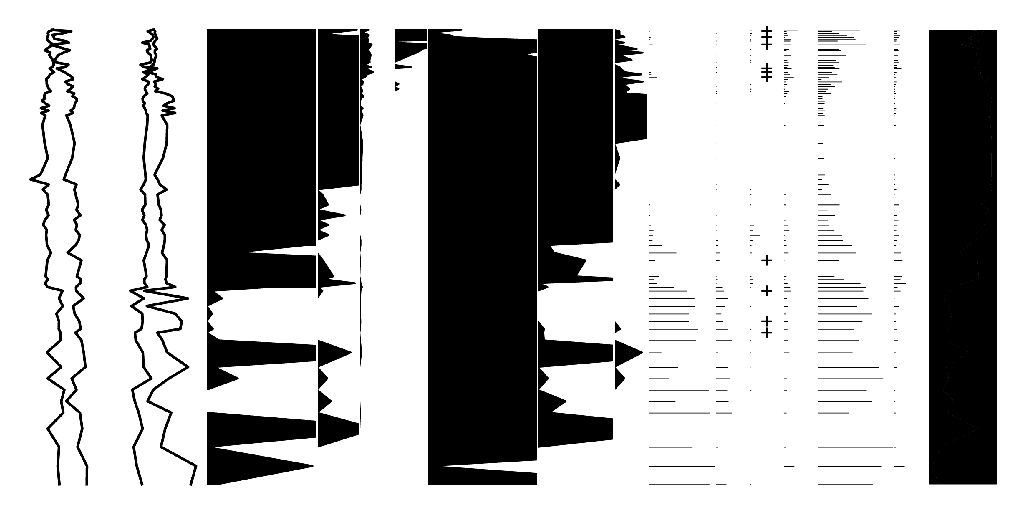
\includegraphics[width=\linewidth]{straditize-figures/sample-diagram-data.pdf}
	\caption[Cleaned binary image of the data part]{Cleaned binary image of the data part of figure \ref{fig:sample-diagram}. Informative features (Y-axes and horizontal lines) have been removed. Exaggerations and occurrences are still in the binary image and are considered separately in section \ref{sec:occurences}.}
	\label{fig:cleaned-sample}
\end{figure}

In order for the automated digitization algorithms to work effectively, \emph{straditize} has to know which pixels contain data (i.e. is part of a line, or a bar), and which pixels are purely informative (such as y-axes or horizontal lines, see fig. \samplediagram[l]). It is necessary for the user to remove informative features from the data part of the diagram to get a clean version that will not confuse the algorithm. Figure \ref{fig:cleaned-sample} shows what this looks like for the sample diagram in figure \samplediagram. \emph{Straditize} has multiple tools to facilitate the removing of informative features, documented in the software and manual, but their applicability depends on the diagram that is subject to digitization.

The most important step of cleaning the diagram is the recognition of the vertical axes (y- axes) that are usually at the start of every column. This is important because it defines the start of the x-axis, and therefore the value assigned to each of the data points, but also because in some cases the line can obscure part of the data itself. For instance, it is possible that the lowest values on the x-axis (see section \ref{sec:straditize-occurences}) are obscured by the vertical line marking the y-axis, making accurate digitization difficult.

\emph{Straditize} therefore has an automatic algorithm to detect vertical axes that tries to minimize the removing of real data pixels. This detection is described by the following algorithm:

Let $C(i)$ be the most frequent color in the pixels of a pixel column $i$, and $D(i)$ the amount of data pixels in this column. A pixel column that is covered by data with more than a user-defined threshold (by default 30 percent of the data part height, see section \ref{sec:straditize-data-part}) is considered as part of a y-axis if 
\begin{itemize}
	\item it is either the first pixel column in the subdiagram with data (i.e. $D(j) = 0$ for $j < i$ and $j$ being larger or equal than the column start of the diagram),
	\item or the dominant color of the pixel column is the same as for the previous pixel column (i.e. $C(i) = C(i-1)$) and the number of data points is approximately the same (i.e. $D(i) \approx  D(i-1)$).
\end{itemize}

This procedure results in one vertical line per column and works independent of whether it is a dotted, dashed or solid line. However, the line width is critical and may vary a lot. If a diagram column contains a filled line (fig. \samplediagram[h]) that merges with the vertical line defining the y-axis, then the algorithm could potentially overestimate the width of the y-axis line. Therefore, we use the median of all of the estimated lines from the various columns as the width of the y-axis line, and reduce the width of each of the lines to this amount.
The algorithm then looks for informative features or other features that appear to be part of the data columns but are not part of the data behind the image. These include small features such as axis tick marks for example, and lighter pixels (i.e. close to white) that are usually a result from the rasterization of the diagram image.
\emph{straditize} then moves the start of the column because it assumes that the starting point for the x-axis (for pollen taxa it would be the 0\% line) is in the middle of the vertical line marking the y-axis.


\subsubsection{Handling low taxon values}  \label{sec:straditize-occurences}

One particular feature often associated with pollen diagrams is the use of vertical exaggeration to help visualize changes in low percentages. Ordinarily, low percentages could be viewed better by changing the x-axis scale for the taxa with low percentages, but with pollen data it is also important to be able to make a visual comparison across all of the taxa listed, including those with high pollen percentages. Therefore, a common scale for all taxa is important. The exaggeration (fig. \samplediagram[j]) usually takes the form of a second line outside of the first, usually representing x5 or x10 exaggeration of the scale presented on the x-axis. This line could be expected to have greater precision than the first for any given pixel resolution, but problems emerge when the value of the exaggerated value exceeds the width of the scale on the x-axis, so that the line marking the exaggerated values is truncated at high values above a certain threshold. 
Another common way to help the reader identify low percentages in pollen diagrams is to use a marker (often a \enquote{+} symbol, fig. \samplediagram[k]) for values below a certain threshold. This can be particularly useful for very low counts where the author wants the reader to be aware that pollen of a certain taxa was found, even if the pollen counted was very low. This is often used for instance with \enquote{important} taxa such as Cereals that can indicate human agricultural activity, and taxa like Larix (Larch) that have notoriously low pollen productivity and where <1.0\% in a pollen diagram may actually represent 20\% of Larix trees in the surrounding landscape. 
For the purpose of digitization, the \emph{straditize} user can either remove these exaggerations, or use some of the functions available in \emph{straditize} to consider both the non-exaggerated and the exaggerated information in the diagram. In the case of the use of symbols to represent values below a threshold, it needs to be decided what value the symbol will represent once it is digitized and turned into numerical data.  In any case, exaggerations and occurences are automatically removed from the image before the diagram is digitized (see next step \ref{sec:straditize-digitize}).

\subsubsection{Digitizing the diagram}  \label{sec:straditize-digitize}

\begin{figure}
	\centering
	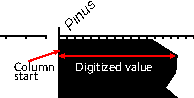
\includegraphics[width=0.5\linewidth]{straditize-figures/sample_diagram_digitize-explanation.pdf}
	\caption[Illustration of the basic digitization strategy of \emph{straditize}]{Illustration of the basic digitization strategy of \emph{straditize}. For each diagram column in the binary image (fig. \ref{fig:cleaned-sample}), we use the pixel that is located furthest to the right on the curve and take the distance to the column start as the digitized value. This is then transformed from the pixel scale into the data units based on the user input.}
	\label{fig:digitize-explanation}
\end{figure}

After removing the informative features (see section \ref{sec:straditize-cleaning}) and exaggerations (see section \ref{sec:straditize-occurences}), \emph{straditize} can automatically digitize the various columns on a pixel basis. In general \emph{straditize} treats every column of the diagram separately and uses different algorithms for the various plotting types:

\begin{description}
	\item[Area and line diagrams] such as those shown in the fig. \samplediagram[f] and fig. \samplediagram[h]  are  digitized  based  on  the  pixel located furthest to the right on the curve in any particular column (illustrated in figure \ref{fig:digitize-explanation}).
	\item[Bar diagrams] as in figure \samplediagram[g] are also digitized based on the the pixel located furthest to the right on the bar in any particular column. Additionally, \emph{straditize} distinguishes between two adjacent bars by using a user defined threshold (by default two pixels). Additionally, it identifies bars that are significantly wider than the others (which would indicate two or more overlapping bars) and then the user can split them manually.
	\item[Stacked diagrams] as in figure \samplediagram[i] have to be digitized manually. The user has to manually distinguish the different areas using the selection tools in \emph{straditize}.
\end{description}

These procedures each result in one value per pixel row in each variable column in the data part. The next step is then to extract only the rows that are necessary to regenerate the diagram, that is, the pixel rows that correspond to the samples.

\subsubsection{Finding the samples}  \label{sec:straditize-samples}
A key function of \emph{straditize} is its ability to identify sample levels in the data, so that measurements of x-axis values in each column for each variable are assigned to the appropriate y-axis sample depth or age across all columns and variables. The search and assignment of sample levels can be done either automatically or manually, and if done automatically, this can also be later edited following manual checking.  

The algorithm is thereby split into two steps:

\begin{enumerate}
	\item For each column: Identify the intervals that contain exactly one sample (the rough locations, i.e. certain consecutive pixel rows in every column where we know that there is a sample, but we do not know where exactly) \label{enum:sample-1}
	\item Align the overlapping intervals between the columns to estimate the exact location \label{enum:sample-2}
\end{enumerate}

The implementation of step \ref{enum:sample-1} necessarily differs between 
bar and area/stacked/line diagrams. With bar diagrams \emph{straditize} uses the bars identified in the
previous digitization step (section \ref{sec:straditize-digitize}) to define these rough sample locations, while for the other diagram types the algorithm looks for local extrema in the graph line, i.e. intervals that are lower or higher than the surrounding areas. This implies that each sample is associated with a local minimum or maximum in at least one of the diagram columns. This holds well for pollen diagrams that usually sum up to 100\% across all of the columns or variables in the diagram, but it is however not generally true for all stratigraphic diagrams.

Step \ref{enum:sample-2} then aligns these rough intervals and uses the overlapping information from the different columns to estimate the exact location of the sample. This is described by the following procedure, where we focus on a simple case of only two diagram columns. Assume that the two columns $i$ and $j$ have a sample in the corresponding overlapping intervals $I_i$ and $I_j$ (i.e. $I_i = \left\{r_{i,1}, r_{i,2}, \ldots\right\}$, and $I_j = \left\{r_{j,1}, r_{j,2}, \ldots\right\}$ with $I_i \cap I_j \neq \emptyset$). To find the exact location, \emph{straditize} distinguishes the following cases:

\begin{description}
	\item[If one of the intervals contains only one pixel row] (i.e. $\left| I_i \right| = 1$ or $\left| I_j \right| = 1$), \emph{straditize} sets the sample at exactly this location
	\item[If each of the intervals contains multiple rows,] \emph{straditize} uses the mean of all the row indices in each of the intervals (i.e. $y = \overline{I_i \cup I_j}$). This then weighs overlapping areas in the intervals above non-overlapping areas.
\end{description}

Finally, samples that are close to each other (by default, closer than 5 pixel rows) are merged together. This is necessary because it may happen that, due to the quality of the diagram image, two rough locations do not exactly overlap although they belong to the same sample.


\setcounter{secnumdepth}{2}
\endgroup

\section{Discussion}  \label{sec:straditize-discussion}

\begin{figure}
	\centering
	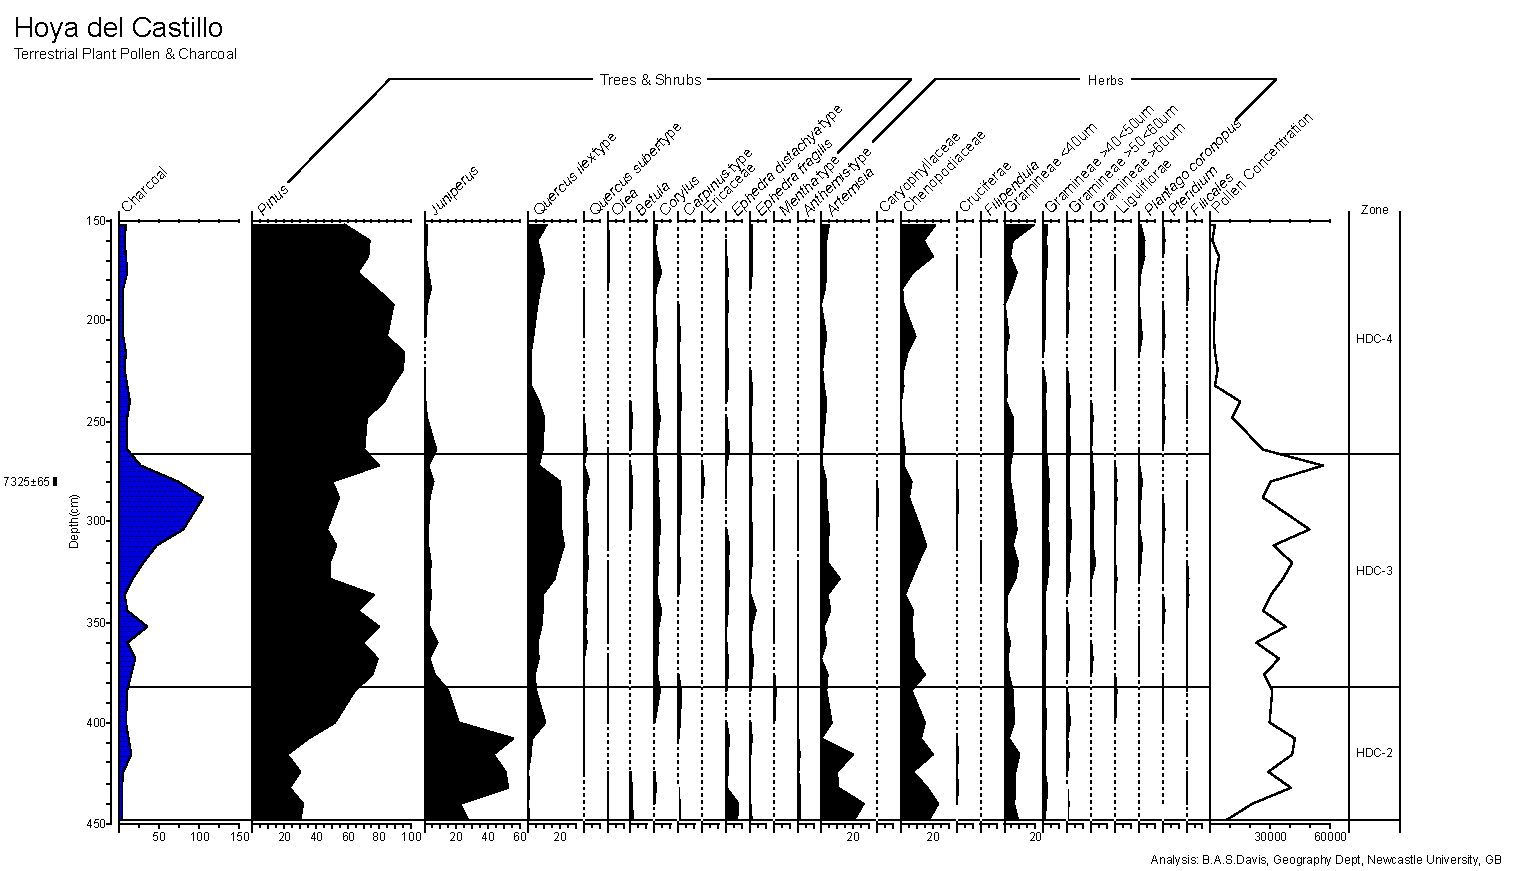
\includegraphics[width=0.45\linewidth]{straditize-figures/hoya-del-castillo.pdf}
	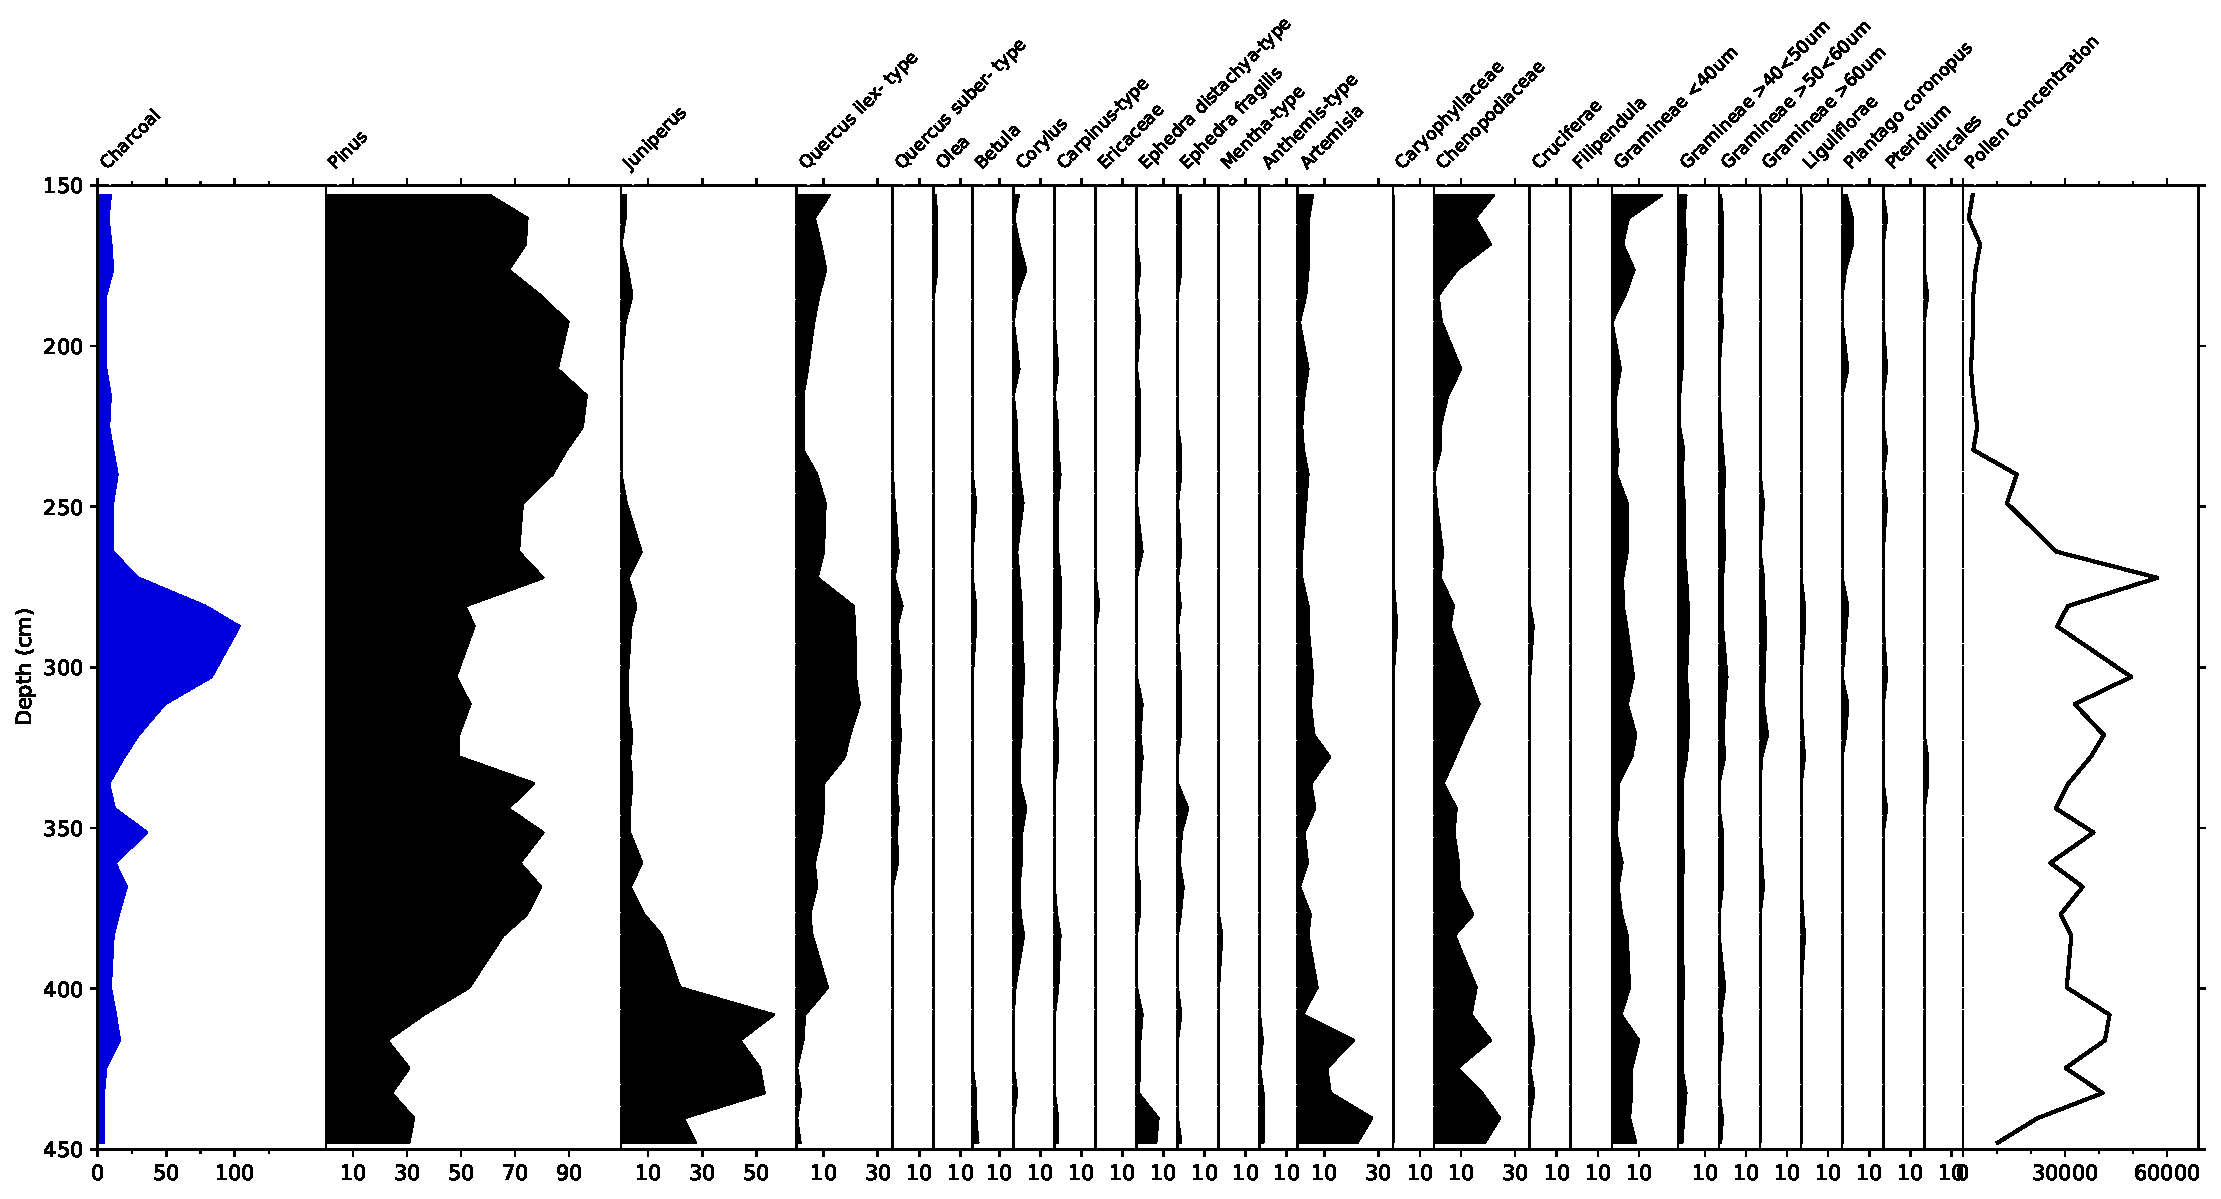
\includegraphics[width=0.45\linewidth]{straditize-figures/hoya-del-castillo-digitized.pdf}
	\caption[Pollen diagram for Hoya del Castillo]{Pollen diagram for Hoya del Castillo after \cite{DavisStevenson2007}. Left,  the original diagram, right, the digitized version obtained (and plotted) using \emph{straditize}.}
	\label{fig:hoya-del-castillo}
\end{figure}

\begin{figure}
	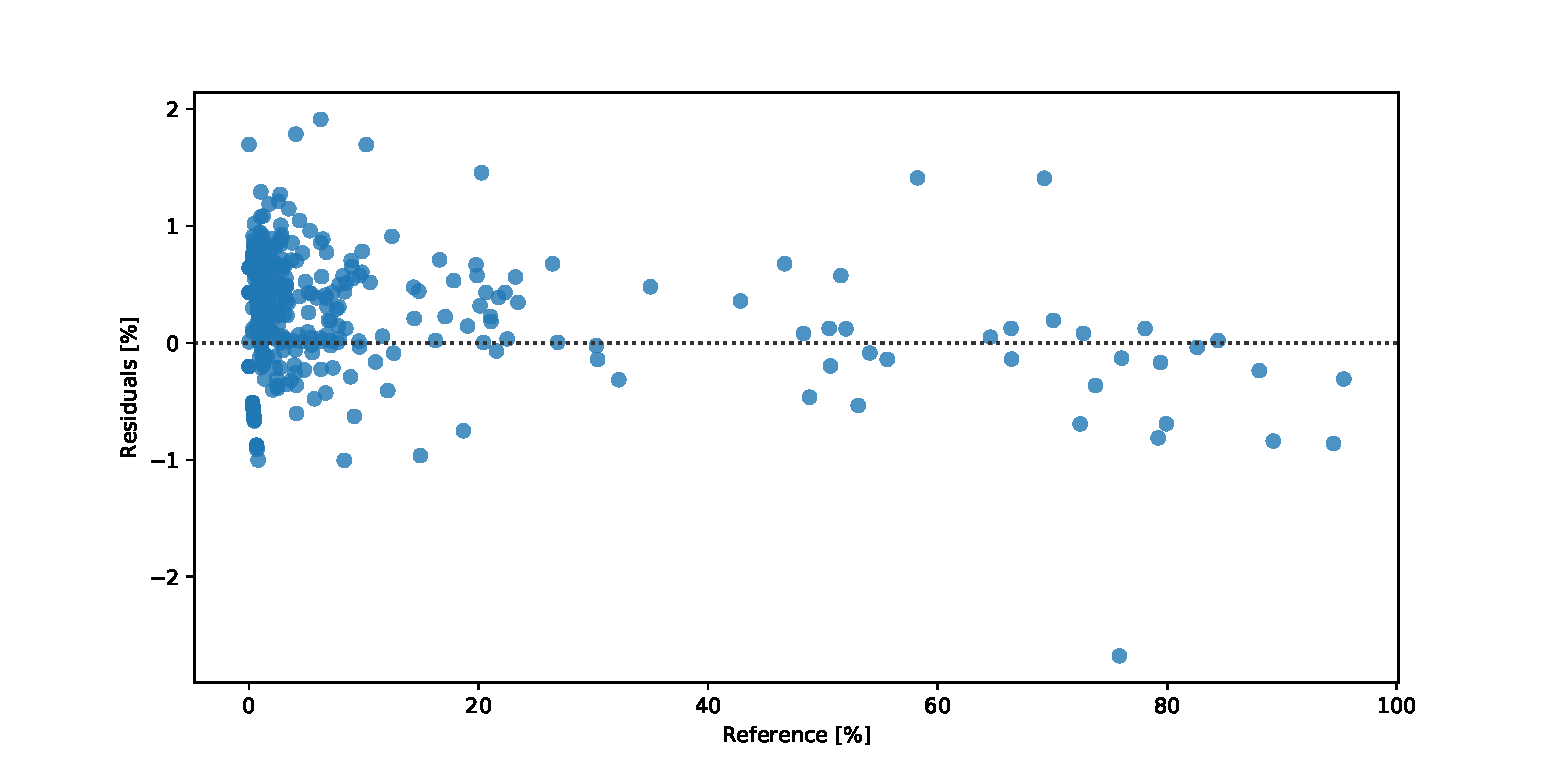
\includegraphics[width=\linewidth]{straditize-figures/resid-plot-hoya-del-castillo.pdf}
	\caption[Residuals plot of the digitized Hoya del Castillo diagram]{A plot of the residuals based on a comparison between the digitized Hoya del Castillo pollen diagram, and the original reference data that was used to generate the diagram (see fig. \ref{fig:hoya-del-castillo}). The y-axis shows the residuals (digitized data percentage minus original reference data percentage) and the x-axis shows the original reference data percentage for Hoya del Castillo. Each dot represents a single pollen sample. The dotted line denotes the one-to-one line where digitization result and reference are the same.}
	\label{fig:hoya-resid}
\end{figure}

As an example of the application of \emph{straditize}, we digitized the Holocene pollen diagram for Hoya del Castillo (Spain) a site in Los Monegros, NE Spain, published by \cite{DavisStevenson2007} (see figure \ref{fig:hoya-del-castillo}). The diagram was generated using the popular pollen diagram plotting software package Tilia\footnote{\url{https://www.tiliait.com/}} \citep{Grimm1988, Grimm1991} and exported as an image with a resolution of 450 dots per inch (dpi). We then followed the strategy described in section \ref{sec:straditize-digitization} to digitize the diagram. First, we selected the data part, then the columns and cleaned the image by removing the y-axes and horizontal lines. Then we digitized the diagram and used the \emph{straditize} sample finding algorithm to extract the sample locations.  

Comparing the digitized data with the original data, we find that \emph{straditize} was able to successfully identify all 34 samples in the diagram. The root mean square error (RMSE) for the depth of each sample digitized from the y-axis and normalized by the range of the vertical axes, is very low and corresponds to an error of 0.2\%. Additionally \emph{straditize} gives a good measure of the individual taxon percentage with the RMSE being only 0.5\%. Nevertheless, \emph{straditize} shows a tendency to overestimate the real percentage. About 43\% of the samples have percentages that are higher than the orginal percentages, whereas only about 10\% have lower percentages (fig. \ref{fig:hoya-resid}), the remainder are exact (and most of the time zero percentage). This is probably due to a systematic bias in the positioning of the exact column start, i.e. 0 start point of the x-axis relative to y-axis baseline, and is something that could be systematically corrected. Overall this error is in the range of less than one percent per sample/taxon.

Irrespective of the performance of the software, other factors will also influence the accuracy of the digitization process. The quality and type of diagram image is very important, especially if the diagram is not of a high pixel resolution, or has poorly aligned and marked axis, or has many closely located samples. But also the skill and experience of the user will have some impact, especially if they are also unfamiliar with the type of data being analyzed and the way that it is commonly presented in a diagram. To help the user evaluate how accurate the digitization process has been, \emph{straditize} also allows the user to plot the digitized data in a way that allows a direct visual comparison with the source diagram (fig. \ref{fig:hoya-del-castillo}) using the stratigraphic visualization features of \textit{psy-strat} \citep{Sommer2019}.

Keeping in mind these many caveats, we generally estimate that \emph{straditize} will allow an experienced user to reliably obtain a numerical estimate through diagram digitization in the order of 1\% of the original data for each sample/variable. In the case of pollen diagrams, this uncertainty should be viewed from the perspective of the inherent uncertainty associated with the counting of each pollen sample. Any pollen count is an estimate of the pollen sample that is displayed on a pollen slide. Although pollen samples are usually displayed as percentages, the reason for this is that the size of the pollen count varies from sample to sample, and percentages allow different samples to be directly compared on a common scale. Each count is a sample of the total pollen assemblage on a slide, and therefore each count represents an estimate of the composition of the total pollen assemblage represented on the slide. The more of that pollen assemblage that is counted, the closer that estimate will be to the actual pollen assemblage. This mean that each pollen sample plotted on a pollen diagram has an inherent uncertainty that is related to the total number of pollen grains counted. The bigger the count, the lower the uncertainty. Typical 0.95 confidence intervals for individual taxa based on a typical pollen count of around 300-500 pollen grains are easily in the order of 2-5\% \citep{Maher1972}.

\section{Conclusions}  \label{sec:straditize-conclusions}
In this paper we present a new open-source software that is capable of greatly reducing the time required to accurately digitize stratigraphic diagrams. These diagrams are characterized by a series of horizontally or vertically aligned diagrams that plot various variables representing the results of the analysis of a series of common samples that are aligned on the same y-axis representing age or depth. The software is currently optimized for use with pollen diagrams, but should work well with any similar type of data plotted in a similar style. The x-axis values can be percentages or absolute values of any kind, and the y-axis could also represent distance down a river of any other linear scale. The program is freely available, well documented with integrated help and training, is written in python, and is also open for adaptation for other uses. 

\printbibliography[heading=subbibintoc]

\end{refsection}